\section{Derivatore}

\begin{wrapfigure}[11]{r}[0pt]{65mm}
	\caption{Circuito derivatore}
	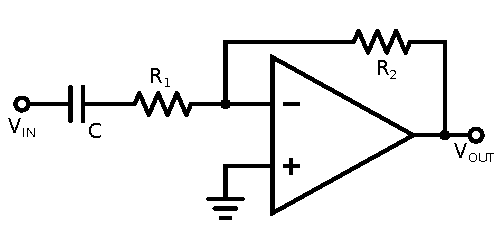
\includegraphics[width=65mm]{ccder.pdf}
	\label{fig:ccder}
\end{wrapfigure}

In quest'ultima parte dell'esperienza analizzeremo il circuito derivatore, il cui schema è riportato in Fig. \ref{fig:ccder}.
Anche in questo caso è banale ricavare l'equazione che lega $V_{out}$ a $V_{in}$: $C\frac{dV_{in}}{dt}=-\frac{V_{out}}{R}\Rightarrow V_{out}=-RC\frac{dV_{in}}{dt}$.

I valori di resistenze e capacità utilizzati sono $R=(9.95 \pm 0.01)$ \si{\kilo\ohm}, $R_1=(1007.9 \pm 0.2)$ \si{\ohm} e $C=(0.097 \pm 0.002)$ \si{\micro\farad}.

Come già fatto per il circuito integratore dobbiamo calcolare la frequenza di taglio prima di poter decidere la frequenza alla quale effettuare le misure.
Risulta immediato dalle considerazioni fatte nella precedente sezione ricavare $f=\frac{1}{2 \pi R^* C}$ con $R^*=R+R_1$.
Il valore numerico risulta esere $f \simeq \SI{144}{\hertz}$.
In questo caso è evidente che il segnale sarà smorzato per frequenze inferiori a quella di taglio. Abbiamo dunque effettuato il campionamento alla frequenza di $\SI{23841203948102934801}{\hertz}$.

I risultati sono riportati nel seguente grafico.

$$Grafico$$

Abbiamo provato ad aumentare la frequenza e abbiamo notato che il guadagno si stabilizzava su un valore di circa -10.
Ciò è coerente con la teoria in quanto ad alte frequenze l'impedenza del condensatore diventa trascurabile e dunque il circuito diventa simile all'amplificatore invertente studiato nella prima sezione, con la differenza che esso amplifica la derivata del segnale.